\documentclass[14pt]{beamer}

\usetheme{Montpellier}
\usecolortheme{beaver}

\usepackage{amsmath, amssymb, ../../vimacros, hyperref, tikz}
\usetikzlibrary{positioning, fit, bayesnet}
\usepackage[round]{natbib}

\hypersetup{breaklinks=true, colorlinks=true, linkcolor=blue, urlcolor=blue, citecolor=blue}

\title{Deep Generative Models}
\author{Philip Schulz and Wilker Aziz\\
\url{https://github.com/philschulz/VITutorial}}
\date{}

\setbeamertemplate{footline}[frame number]

\begin{document}

\begin{frame}
\maketitle
\end{frame}

\frame{\tableofcontents}

\section{Generative Models}
\frame{\tableofcontents[currentsection]}

\begin{frame}{Recap: Generative Models}
Joint distribution over observed data $ x $ and latent variables $ Z $.
\begin{equation*}
p(x,z|\alpha) = \overbrace{p(x|z,\alpha)}^{\text{likelihood}} \underbrace{p(z|\alpha)}_{\text{prior}}
\end{equation*} 
The likelihood and prior are often standard distributions (Gaussian, Bernoulli) with simple dependence on conditioning
information.
\end{frame}

\begin{frame}{Recap: Variational Inference}
\begin{block}{Objective}
\begin{equation*}
\underset{q(z)}{\max}~\E{\log p(x,z)} + \Ent{q(z)}
\end{equation*}
\begin{itemize}
\item The ELBO is a lower bound on $ \log p(x) $
\item Mean field assumption: $ q(z) = \prod_{i=1}^{N}q(z_{i}) $
\end{itemize}
\end{block}
\end{frame}

\section{First Attempt: Log-linear Models}
\frame{\tableofcontents[currentsection]}

\begin{frame}{Feature-rich Generative Models}
Let us assume that $ z $ has internal structure (features). How can we exploit that?
\begin{block}{First Idea}
Make $ p(x|z,\alpha) $ a log-linear model.
\begin{itemize}
\item Only discrete data
\item Trainable with EM if we can efficiently enumerate $ \mathcal{X} $ and $ \mathcal{Z} $.
\end{itemize}
\end{block}
\end{frame}

\begin{frame}{Log-linear Model}
Let us treat $ z $ as observed.
\begin{equation*}
p(x|z,\alpha\alert{=w}) = \frac{\exp\left(w^{\top}f(x,z)\right)}{\sum_{x\in \mathcal{X}}\exp\left(w^{\top}f(x,z)\right)}
\end{equation*}
\pause
\begin{block}{Weight Gradient}
\begin{equation*}
\frac{d}{dw}\log p(x|z,w) = f(x,z) - \E{f(X,z)|z,w} 
\end{equation*}
\pause
Updates need to be performed iteratively.
\end{block}
\end{frame}

\begin{frame}{Log-linear model with latent variables}
Now let us treat $ z $ as latent.
\pause
\begin{block}{Model}
\begin{equation*}
p(x,z|w) = \underbrace{\frac{\exp\left(w^{\top}f(x,z)\right)}{\sum_{x\in \mathcal{X}}\exp\left(w^{\top}f(x,z)\right)}}_{p(x|z, w)} 
\times \underbrace{p(z)}_{arbitrary}
\end{equation*}
\end{block}
\end{frame}

\begin{frame}{Log-linear model with latent variables}
\begin{block}{Posterior}
\begin{align*}
p(z|x,w) \onslide<2->{= \frac{p(x,z|w)}{p(x|w)}} \onslide<3->{= \frac{p(x,z|w)}{\sum_{z} p(x,z|w)} =} \\
\onslide<4>{\dfrac{\frac{\exp\left(w^{\top}f(x,z)\right)}{\sum_{x\in \mathcal{X}}\exp\left(w^{\top}f(x,z)\right)} \times p(z)}
{\sum_{z} \frac{\exp\left(w^{\top}f(x,z)\right)}{\sum_{x\in \mathcal{X}}\exp\left(w^{\top}f(x,z)\right)} \times p(z)}}
\end{align*}
\end{block}
\end{frame}

\begin{frame}{Log-linear model with latent variables}
\begin{block}{Weight Gradient (treat $ p(z|x,w) $ as fixed)}
\begin{small}
\begin{align*}
&\frac{d}{dw}\E[p(z|x,w)]{\log p(x,z|w)} = \\ 
&\onslide<2->{\frac{d}{dw}\sum_{z}p(z|x,w) \log p(x,z|w) =} \\
&\onslide<3->{\sum_{z}p(z|x,w)  \frac{d}{dw}\log p(x,z|w) =} \\
&\onslide<4>{\sum_{z}p(z|x,w) \left( \frac{d}{dw}\log p(x|z,w) + \frac{d}{dw} p(z) \right)}
\end{align*}
\end{small}
\end{block}
\end{frame}

\begin{frame}{Log-linear model with latent variables}
\begin{block}{Weight Gradient (treat $ p(z|x,w) $ as fixed)}
\begin{small}
\begin{align*}
&\frac{d}{dw}\E[p(z|x,w)]{\log p(x,z|w)} = \\ 
&\frac{d}{dw}\sum_{z}p(z|x,w) \log p(x,z|w) = \\
&\sum_{z}p(z|x,w)  \frac{d}{dw}\log p(x,z|w) = \\
&\sum_{z}p(z|x,w) \left( \alert{\overbrace{\frac{d}{dw} \log p(x|z,w)}^{\text{We've already solved this!}}} + \overbrace{\frac{d}{dw} p(z)}^{\text{0}} \right)
\end{align*}
\end{small}
\end{block}
\end{frame}

\begin{frame}{Log-linear model with latent variables}
\begin{block}{Weight Gradient (treat $ p(z|x,w) $ as fixed)}
\begin{align*}
&\frac{d}{dw}\E[p(z|x,w)]{\log p(x,z|w)} = \\ 
&\E[p(z|x,w)]{f(x,Z)|x,w} - \E[p(z|x,w)]{\E{(f(X,Z)|Z,w}}
\end{align*}
\end{block}
\pause
\begin{block}{Procedurally}
\begin{small}
\center{E\_count($f(x,z)$) - \{ E\_count($ f(x,z) $) $ \times  \E{f(X,z)|z,w} $ \}}
\end{small}
\end{block}
\end{frame}

\begin{frame}{EM}
\begin{itemize}
\item[E-step] $ p(z|x,w) = \frac{p(x,z|w)}{\sum_{z} p(x,z|w)} $
in $ \mathcal{O}(|\mathcal{X}|\times |\mathcal{Z}|) $
\item[M-step] Iteratively optimise $ w $ to match E\_count($x,z$) with E\_count($ x,z $) $ \times  \E{X|z,w} $ 
\end{itemize}
\begin{block}{Restrictions}
\begin{itemize}
\item Only log-linear models
\item Scales badly
\end{itemize}
\end{block}
\end{frame}

\section{Second Attempt: Wake-Sleep}
\frame{\tableofcontents[currentsection]}

\begin{frame}{Wake-sleep Algorithm}
\begin{itemize}
\item Generalise latent variables to Neural Networks
\item Train generative neural model
\item Use variational inference! (kind of)
\end{itemize}
\end{frame}

\begin{frame}{Wake-sleep Architecture}
2 Neural Networks:
\begin{itemize}
\pause
\item A generation network to model the data (the one we want to optimise) -- parameters: $ \theta $
\pause
\item An inference (recognition) network (to model the latent variable) -- parameters: $ \lambda $
\pause
\item Original setting: binary hidden units
\pause
\item Training is performed in a ``hard EM'' fashion
\end{itemize}
\end{frame}

\begin{frame}{Wake-sleep Training}
\textbf{Wake Phase} \\
\begin{itemize}
\item Use inference network to sample hidden unit setting $ z $ from $ q(z|x,\lambda) $
\item Update generation parameters $ \theta $ to maximize liklelihood of data given latent state $ p(x|z,\theta) $
\end{itemize}
\pause
\textbf{Sleep Phase}
\begin{itemize}
\item Produce dream sample $ \tilde{x} $ from random hidden unit $ z $
\item Update inference parameters $ \lambda $ to maximize probability of latent state $ q(z|\tilde{x},\lambda) $
\end{itemize}
\end{frame}

\begin{frame}{Wake Phase Objective}
Assumes latent state $ z $ to be fixed random draws from $ q(z|x,\lambda) $.
\begin{equation*}
\max_{\theta}~ \log p(x|z,\theta) 
\end{equation*}
This is simply supervised learning with imputed latent data!
\end{frame}

\begin{frame}{Wake Phase Sampling}
\begin{figure}
\center
\begin{tikzpicture}
\node[draw, circle] (z3) {$ z_{3} $};

\node[draw, circle, below left =of z3] (z1) {$ z_{1} $};
\node[draw, circle, below right = of z3] (z2) {$ z_{2} $};

\node[draw, rectangle,  below left= of z1] (in1) {$ x_{1} $};
\node[draw, rectangle, below left=of z2] (in2) {$ x_{2} $}; 
\node[draw, rectangle, below right= of z2] (in3) {$ x_{3} $};
\end{tikzpicture}
\end{figure}
\end{frame}

\begin{frame}{Wake Phase Sampling}
\begin{figure}
\center
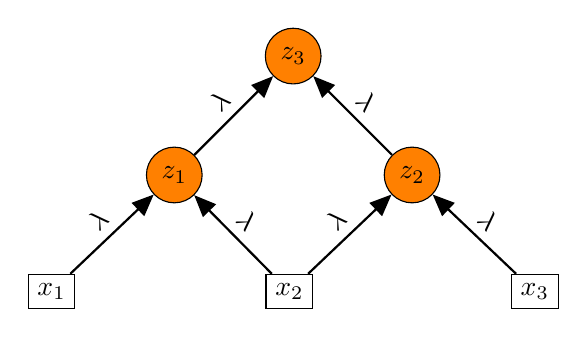
\begin{tikzpicture}
\node[draw, circle, fill=orange] (z3) {$ z_{3} $};

\node[draw, circle, fill=orange, below left =of z3] (z1) {$ z_{1} $};
\node[draw, circle, fill=orange, below right = of z3] (z2) {$ z_{2} $};

\node[draw, rectangle,  below left= of z1] (in1) {$ x_{1} $};
\node[draw, rectangle, below left=of z2] (in2) {$ x_{2} $}; 
\node[draw, rectangle, below right= of z2] (in3) {$ x_{3} $};

\draw[->, thick] (in1) -- (z1) node[midway, above, rotate=45] {$ \lambda $};
\draw[->, thick] (in2) -- (z1) node[midway, above, rotate=315] {$ \lambda $};
\draw[->, thick] (in2) -- (z2) node[midway, above, rotate=45] {$ \lambda $};
\draw[->, thick] (in3) -- (z2) node[midway, above, rotate=315] {$ \lambda $};
\draw[->, thick] (z1) -- (z3) node[midway, above, rotate=45] {$ \lambda $};
\draw[->, thick] (z2) -- (z3) node[midway, above, rotate=315] {$ \lambda $};
\end{tikzpicture}
\end{figure}
\end{frame}

\begin{frame}{Wake Phase Update}
\begin{figure}
\center
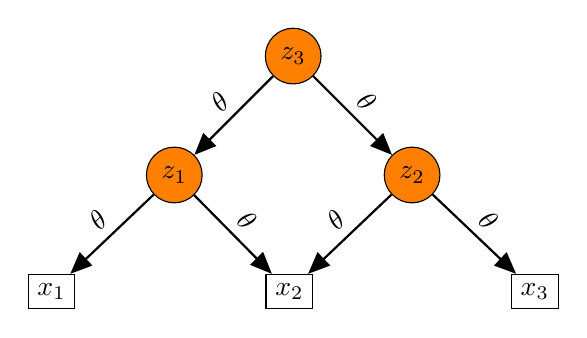
\begin{tikzpicture}
\node[draw, circle, fill=orange] (z3) {$ z_{3} $};

\node[draw, circle, fill=orange, below left =of z3] (z1) {$ z_{1} $};
\node[draw, circle, fill=orange, below right = of z3] (z2) {$ z_{2} $};

\node[draw, rectangle,  below left= of z1] (in1) {$ x_{1} $};
\node[draw, rectangle, below left=of z2] (in2) {$ x_{2} $}; 
\node[draw, rectangle, below right= of z2] (in3) {$ x_{3} $};

\draw[->, thick] (z1) -- (in1) node[midway, above, rotate=45] {$ \theta $};
\draw[->, thick] (z1) -- (in2) node[midway, above, rotate=315] {$ \theta $};
\draw[->, thick] (z2) -- (in2) node[midway, above, rotate=45] {$ \theta $};
\draw[->, thick] (z2) -- (in3) node[midway, above, rotate=315] {$ \theta $};
\draw[->, thick] (z3) -- (z1) node[midway, above, rotate=45] {$ \theta $};
\draw[->, thick] (z3) -- (z2) node[midway, above, rotate=315] {$ \theta $};
\end{tikzpicture}
\end{figure}
\end{frame}

\begin{frame}{Sleep Phase Objective}
Assumes fake data $ \tilde{x} $ and latent variables $ z $ to be fixed random draw from $ p(x,z|\theta) $.
\begin{equation*}
\min_{\lambda}~  \E[q(z|\tilde{x},\lambda)]{\log p(\tilde{x},z|\theta)} + \Ent{q(z|\tilde{x},\lambda)}
\end{equation*}
\end{frame}

\begin{frame}{Sleep Phase Sampling}
\begin{figure}
\center
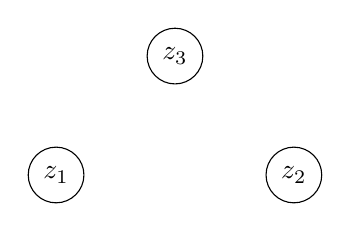
\begin{tikzpicture}
\node[draw, circle] (z3) {$ z_{3} $};

\node[draw, circle, below left =of z3] (z1) {$ z_{1} $};
\node[draw, circle, below right = of z3] (z2) {$ z_{2} $};
\end{tikzpicture}
\end{figure}
\end{frame}

\begin{frame}{Sleep Phase Sampling}
\begin{figure}
\center
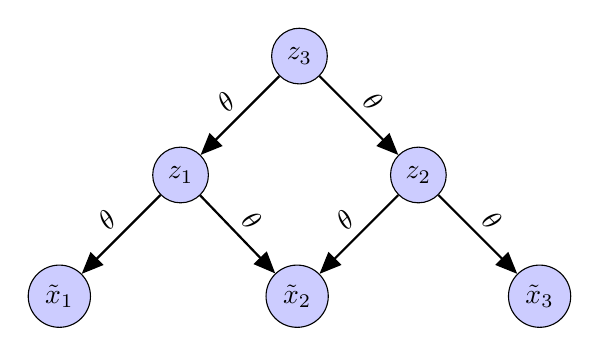
\begin{tikzpicture}
\node[draw, circle, fill=blue!20] (z3) {$ z_{3} $};

\node[draw, circle, fill=blue!20, below left =of z3] (z1) {$ z_{1} $};
\node[draw, circle, fill=blue!20, below right = of z3] (z2) {$ z_{2} $};

\node[draw, circle, fill=blue!20, below left= of z1] (in1) {$ \tilde{x}_{1} $};
\node[draw, circle, fill=blue!20, below left=of z2] (in2) {$ \tilde{x}_{2} $}; 
\node[draw, circle, fill=blue!20, below right= of z2] (in3) {$ \tilde{x}_{3} $};

\draw[->, thick] (z1) -- (in1) node[midway, above, rotate=45] {$ \theta $};
\draw[->, thick] (z1) -- (in2) node[midway, above, rotate=315] {$ \theta $};
\draw[->, thick] (z2) -- (in2) node[midway, above, rotate=45] {$ \theta $};
\draw[->, thick] (z2) -- (in3) node[midway, above, rotate=315] {$ \theta $};
\draw[->, thick] (z3) -- (z1) node[midway, above, rotate=45] {$ \theta $};
\draw[->, thick] (z3) -- (z2) node[midway, above, rotate=315] {$ \theta $};
\end{tikzpicture}
\end{figure}
\end{frame}

\begin{frame}{Sleep Phase Update}
\begin{figure}
\center
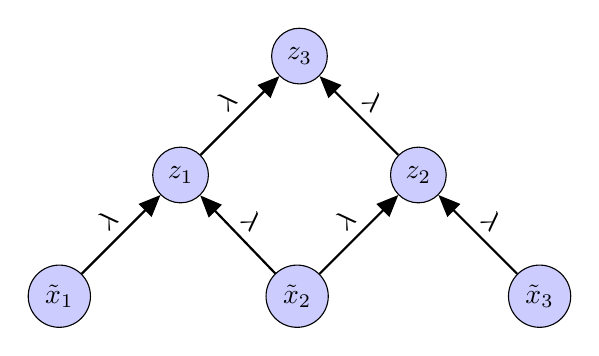
\begin{tikzpicture}
\node[draw, circle, fill=blue!20] (z3) {$ z_{3} $};

\node[draw, circle, fill=blue!20, below left =of z3] (z1) {$ z_{1} $};
\node[draw, circle, fill=blue!20, below right = of z3] (z2) {$ z_{2} $};

\node[draw, circle, fill=blue!20, below left= of z1] (in1) {$ \tilde{x}_{1} $};
\node[draw, circle, fill=blue!20, below left=of z2] (in2) {$ \tilde{x}_{2} $}; 
\node[draw, circle, fill=blue!20, below right= of z2] (in3) {$ \tilde{x}_{3} $};

\draw[->, thick] (in1) -- (z1) node[midway, above, rotate=45] {$ \lambda $};
\draw[->, thick] (in2) -- (z1) node[midway, above, rotate=315] {$ \lambda $};
\draw[->, thick] (in2) -- (z2) node[midway, above, rotate=45] {$ \lambda $};
\draw[->, thick] (in3) -- (z2) node[midway, above, rotate=315] {$ \lambda $};
\draw[->, thick] (z1) -- (z3) node[midway, above, rotate=45] {$ \lambda $};
\draw[->, thick] (z2) -- (z3) node[midway, above, rotate=315] {$ \lambda $};
\end{tikzpicture}
\end{figure}
\end{frame}

\begin{frame}{Wake-sleep Algorithm}
\textbf{Advantages}
\begin{itemize}
\item Simple layer-wise updates
\item Amortised inference: all latent variables are inferred from the same weights $ \lambda $
\end{itemize}
\pause
\textbf{Drawbacks}
\begin{itemize}
\item Inference and generative networks are trained on different objectives
\item Inference weights $ \lambda $ are updated on fake data $ \tilde{x} $
\item Generative weights are bad initially, giving wrong signal to the updates of $ \lambda $
\end{itemize}
\end{frame}

\section{This is how we do: Variational Autoencoders}
\frame{\tableofcontents[currentsection]}

\begin{frame}{Generative Model with NN Likelihood}
\begin{block}{Goal}
Define model $ p(x,z|\theta) = p(x|z,\theta)p(z) $ where the likelihood $ p(x|z,\theta) $ is given by a neural
network. (We fix $ p(z) $ for simplicity.)
\end{block}
\pause
\begin{block}{Problem}
$ p(x) = \intl{p(x|z,\theta) p(z)}{z} $ is hard to compute.
\end{block}
\end{frame}

\begin{frame}{Generative Model with NN Likelihood}
\begin{block}{Goal}
Define model $ p(x,z|\theta) = p(x|z,\theta)p(z) $ where the likelihood $ p(x|z,\theta) $ is given by a neural
network. (We fix $ p(z) $ for simplicity.)
\end{block}
\begin{block}{Problem}
$ p(x) = \intl{\alert{\underbrace{p(x|z,\theta)}_{\substack{\text{highly} \\  \text{non-linear!}}}} p(z)}{z} $ is hard to compute.
\end{block}
\end{frame}

\begin{frame}{Generative Model with NN Likelihood}
\begin{block}{Solution: VI}
\begin{small}
\begin{equation*}
\begin{aligned}
\log p(x) &\geq \overbrace{\E[q(z|x,\lambda)]{\log p(x,z|\theta)} + \Ent{q(z|x,\lambda)}}^{\ELBO} \\ 
\pause
&= \E[q(z|x,\lambda)]{\log p(x|z,\theta) + \log p(z)} + \Ent{q(z|x,\lambda)} \\ \pause
&= \E[q(z|x,\lambda)]{\log p(x|z,\theta)} - \KL{q(z|x,\lambda)}{p(z)}
\end{aligned}
\end{equation*}
\end{small}
\end{block}
\end{frame}

\begin{frame}{Generative Model with NN Likelihood}
\begin{block}{Solution: VI}
\begin{small}
\begin{align*}
\log p(x) &\geq \overbrace{\E[q(z|x,\lambda)]{\log p(x,z|\theta)} + \Ent{q(z|x,\lambda)}}^{\ELBO} \\
&= \E[q(z|x,\lambda)]{\log p(x|z,\theta) + \log p(z)} + \Ent{q(z|x,\lambda)} \\
&= \E[q(z|x,\lambda)]{\log p(x|z,\theta)} - \alert{\underbrace{\KL{q(z|x,\lambda)}{p(z)}}_{\substack{\text{assume analytical} \\ \text{(true for exponential families)}}}}
\end{align*}
\end{small}
\end{block}
\end{frame}

\begin{frame}{Generative Model with NN Likelihood}
\begin{block}{Solution: VI}
\begin{small}
\begin{align*}
\log p(x) &\geq \overbrace{\E[q(z|x,\lambda)]{\log p(x,z|\theta)} + \Ent{q(z|x,\lambda)}}^{\ELBO} \\
&= \E[q(z|x,\lambda)]{\log p(x|z,\theta) + \log p(z)} + \Ent{q(z|x,\lambda)} \\ 
&= \alert{\underbrace{\E[q(z|x,\lambda)]{\log p(x|z,\theta)}}_{\text{approximate by sampling}}} - \underbrace{\KL{q(z|x,\lambda)}{p(z)}}_{\substack{\text{assume analytical} \\ \text{(true for exponential families)}}}
\end{align*}
\end{small}
\end{block}
\end{frame}

\begin{frame}{Generation Network Gradient}
\begin{equation*}
\begin{aligned}
&\frac{d}{d\theta}\E[q(z|x,\lambda)]{\log p(x|z,\theta)} - \overbrace{\KL{q(z|x,\lambda)}{p(z)}}^{constant} \\ \pause 
&=\E[q(z|x,\lambda)]{\frac{d}{d\theta}\log p(x|z,\theta)} \\ \pause
&\overset{\text{MC}}{\approx} \frac{1}{S}\sum_{i=1}^{S}
\frac{d}{d\theta} \log p(x|z_{i},\theta)
\end{aligned}
\end{equation*}
\pause
\center{Note: $ q(z|x,\lambda) $ does not depend on $ \theta $.}
\end{frame}

\begin{frame}{Inference Network Gradient}
\begin{equation*}
\begin{aligned}
&\frac{d}{d\lambda}\left[\E[q(z|x,\lambda)]{\log p(x|z,\theta)} - \KL{q(z|x,\lambda)}{p(z)} \right] \\ \pause
=&\frac{d}{d\lambda}\E[q(z|x,\lambda)]{\log p(x|z,\theta)} - \underbrace{\frac{d}{d\lambda}\KL{q(z|x,\lambda)}{p(z)}}_{\text{analytical computation}} \\
\end{aligned}
\end{equation*}
\pause
\center{The first term again requires approximation by sampling}
\end{frame}

\begin{frame}{Inference Network Gradient}
\begin{align*}
&\frac{d}{d\lambda}\E[q(z|x,\lambda)]{\log p(x|z,\theta)} \\
&= \frac{d}{d\lambda} \intl{q(z|x,\lambda)\log p(x|z,\theta)}{z}
\end{align*}
\pause
\begin{block}{MC estimator non-differentiable}
\begin{itemize}
\pause
\item Sampling $ z $ neglects $ \frac{d}{d\lambda} q(z|x,\lambda) $
\pause
\item Differentiating $ q(z|x,\lambda) $ breaks the expectation
\end{itemize}
\end{block}
\end{frame}

\begin{frame}{Inference Network Gradient}
\begin{block}{Reparametrisation trick}
Find a transformation $ h: z \mapsto \epsilon $ such that $ \epsilon $ does not depend on $ \lambda $.
\begin{itemize}
\item $ h(z, \lambda) $ needs to be invertible
\item $ h(z, \lambda) $ needs to be differentiable
\pause
\item $ h(z, \lambda) = \epsilon $
\item $ h^{-1}(\epsilon, \lambda) = z $ 
\end{itemize}
\end{block}
\end{frame}

\begin{frame}{Gaussian Transformation}
\pause
\textbf{Affine property}
\begin{equation*}
Ax + b \sim \NDist{\mu + b}{A\Sigma A^{T}} \text{ for } x \sim \NDist{\mu}{\Sigma}
\end{equation*}
\pause
\textbf{Special case}
\begin{equation*}
Ax + b \sim \NDist{b}{A A^{T}} \text{ for } x \sim \NDist{0}{\IMatrix}
\end{equation*}
\pause
\textbf{Gaussian transformation}
\begin{align*}
h(z, \lambda) &= \frac{z - \mu(x,\lambda)}{ \sigma(x, \lambda) } = \epsilon \sim \NDist{0}{\IMatrix} \\
h^{-1}(\epsilon, \lambda) &= \mu(x,\lambda) + \sigma(x, \lambda) \odot \epsilon~~~\epsilon \sim \NDist{0}{\IMatrix}
\end{align*}
\end{frame}

\begin{frame}{Inference Network Gradient}
\begin{equation*}
\begin{aligned}
&= \frac{d}{d\lambda} \intl{q(z|x,\lambda)\log p(x|z,\theta)}{z} \\ \pause
&= \frac{d}{d\lambda} \intl{\alert{q(\epsilon)} \loga{ p(x | \alert{\overbrace{h^{-1}(\epsilon, \lambda)}^{=z}},\theta)}}{\alert{\epsilon}} \\ \pause
&= \intl{q(\epsilon) \frac{d}{d\lambda} \left[ \log p(x| \overbrace{h^{-1}(\epsilon, \lambda)}^{=z}, \theta)\right] }{\epsilon}
\end{aligned}
\end{equation*}
\end{frame}

\begin{frame}{Inference Network Gradient}
\begin{equation*}
\begin{aligned}
&= \intl{q(\epsilon) \frac{d}{dz} \log p(x| \overbrace{h^{-1}(\epsilon, \lambda)}^{=z}, \theta) \times \frac{d}{d\lambda} h^{-1}(\epsilon, \lambda)}{\epsilon}  \\ \pause
&= \E[q(\epsilon)]{\frac{d}{dz} \log p(x| \overbrace{h^{-1}(\epsilon, \lambda)}^{=z}, \theta)\times \frac{d}{d\lambda} h^{-1}(\epsilon, \lambda)}\\ \pause
&\overset{\text{MC}}{\approx} \frac{1}{S}\sum_{i=1}^{S} \frac{d}{dz} \log p(x| \overbrace{h^{-1}(\epsilon, \lambda)}^{=z}, \theta) \times \frac{d}{d\lambda} h^{-1}(\epsilon, \lambda)
\end{aligned}
\end{equation*}
\end{frame}

\begin{frame}{Derivatives of Gaussian transformation}
Recall:
$$ h^{-1}(\epsilon, \lambda) = \mu(x,\lambda) + \sigma(x,\lambda) \odot \epsilon \ . $$
\pause
This gives us 2 gradient paths.
\pause
\begin{align*}
\frac{d h^{-1}(\epsilon, \lambda)}{d\mu(x,\lambda)} = \frac{d}{d\mu(x,\lambda)}\left[ \mu(x,\lambda) + \sigma(x,\lambda) \odot \epsilon \right] = 1 \\
\frac{d h^{-1}(\epsilon, \lambda)}{d\sigma(x,\lambda)} = \frac{d}{d\sigma(x,\lambda)}\left[ \mu(x,\lambda) + \sigma(x,\lambda) \odot \epsilon \right] = \epsilon
\end{align*}
\end{frame}

\begin{frame}{Gaussian KL}
\begin{block}{ELBO}
\begin{equation*}
\E[q(z|x,\lambda)]{\log p(x|z,\theta)} - \KL{q(z|x,\lambda)}{p(z)}
\end{equation*}
\end{block}
\pause
Analytical computation of $ -\KL{q(z|x,\lambda)}{p(z)} $:
\begin{equation*}
\frac{1}{2}\sum_{i=1}^{N}\left(1 + \loga{\sigma^{2}_{i}} -
\mu_i - \sigma^{2}_{i} \right)
\end{equation*}
\end{frame}

\begin{frame}{Computation Graph}
\begin{figure}
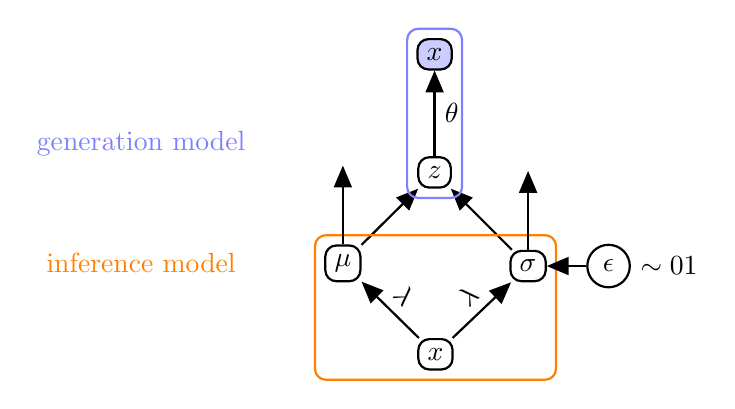
\begin{tikzpicture}[node distance=1cm]
\node[rectangle, draw, rounded corners, thick] (input) {$x$};
\node[rectangle, draw, rounded corners, thick, above left=of input] (mu) {$ \mu $};
\node[rectangle, draw, rounded corners, thick, above right=of input] (var) {$ \sigma $};
\node[rectangle, draw, rounded corners, thick, above right= of mu] (z) {$ z $};
\node[rectangle, fill=blue!20, thick, above of= z, rounded corners, draw, node distance=1.5cm] (output) {$ x $};

\draw[->, thick] (input) -- (mu) node[midway, above, rotate=315] {$ \lambda $};
\draw[->, thick] (input) -- (var) node[midway, above, rotate=45] {$ \lambda $};
\draw[->, thick] (mu) edge (z);
\draw[->, thick] (var) edge (z);
\draw[->, thick] (z) -- (output) node[midway, right] {$ \theta $};

\pause
\node[draw=orange, thick, rectangle, fit= (input) (mu) (var), rounded corners] {};
\node[left= of mu] (inference) {\textcolor{orange}{inference model}};

\pause
\node[draw=blue!50, thick, rectangle, fit= (z) (output), rounded corners] {};
\node[above= of inference] (generation) {\textcolor{blue!50}{generation model}};

\pause
\node[circle, draw, thick ,right =of var, xshift=-.5cm] (epsilon) {$ \epsilon $};
\node[right = of epsilon, xshift=-1cm] (stdNormal) {$ \sim \NDist{0}{1} $};
\draw[->, thick] (epsilon) edge (var);

\pause
\node[above= of mu] (KLmu) {$ \KullbackLeibler $};
\draw[->, thick] (mu) edge (KLmu);
\node[above= of var] (KLvar) {$ \KullbackLeibler $};
\draw[->, thick] (var) edge (KLvar);
\end{tikzpicture}
\end{figure}
\end{frame}

\begin{frame}{Example}
\begin{itemize}
\item Data: binary mnist
\item Likelihood: product of Bernoullis
\begin{itemize}
\item Let $ \phi = \sigma(\text{NN}(z)) $
\item $ \prod_{i=1}^{N} p(x_{i}|\phi) = \prod_{i=1}^{N} \phi^{x_{i}} \times (1-\phi)^{1-x_{i}} $
\end{itemize}
\item Prior over $ z $: $\NDist{0}{1}$
\item $ q(z|x,\lambda) = \NDist{\mu(x,\lambda)}{\sigma(x,\lambda)^{2}} $
\item $ \mu(x, \lambda) = \text{NN}_{\mu}(x; \lambda) $
\item $ \sigma(x, \lambda) = \text{NN}_{\sigma}(x; \lambda) $
\end{itemize}
\pause
\begin{block}{Mean Field assumption}
Variational approximation factorises over latent dimensions.
\end{block}
\end{frame}

\begin{frame}{Graphical Model}
	
	\begin{columns}
	\begin{column}{0.2\textwidth}
	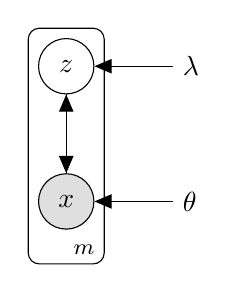
\begin{tikzpicture}
    % Define nodes
    \node[latent]		(z)		{$ z $};
    \node[obs, below = of z]		(x)		{$ x $};
    \node[right = of x]		(theta)		{$ \theta $};
    
    % Connect nodes
    \edge{z,theta}{x};
    
    % add plates
    \plate {x-sentence} {(x)(z)} {$ m $};
   
    \node[right = of z]		(lambda)		{$ \lambda $};   
    \edge[dashed, bend right]{x}{z};
    \edge{lambda}{z};
    \end{tikzpicture}
    \end{column}
    \begin{column}{0.7\textwidth}
    	\begin{itemize}
			\item approximate posterior \\ 
			\begin{small}
			$q(z|x,\lambda) = \NDist{\mu(x,\lambda)}{\sigma(x,\lambda)^{2}}$
			\end{small} \pause
			\item where 
			\begin{itemize}
				\item $\mu(x, \lambda) = \text{NN}_{\mu}(x; \lambda) $ \\
				e.g. $\mu(x, \lambda) = W^{(u)} x + b^{(u)}$ \pause
				\item $\sigma(x, \lambda) = \exp(\text{NN}_{\sigma}(x; \lambda))$ \\
				e.g. $\sigma(x, \lambda) = \loga{ 1 + \exp \left( W^{(v)} x + b^{(v)} \right)}$ \pause
			  \item $\lambda=(W^{(u)}, W^{(v)}, b^{(u)}, b^{(v)})$
		   \end{itemize}
	  \end{itemize}
    \end{column}
    \end{columns}
\end{frame}

\begin{frame}{Variational Autoencoder}
\textbf{Advantages}
\begin{itemize}
\item Backprop training
\item Easy to implement
\item Posterior inference possible
\item One objective for both NNs
\end{itemize}
\pause
\textbf{Drawbacks}
\begin{itemize}
\item Discrete latent variables are difficult
\item Optimisation may be difficult with several latent variables
\end{itemize}
\end{frame}

\begin{frame}{Summary}
\begin{itemize}
\item When $ |\mathcal{X}| $ and $ |\mathcal{Z}| $ are not too large, we can do EM with features
\item Otherwise use VI with simple approximation
\item Wake-Sleep: train inference and generation networks with separate objectives
\item VAE: train both networks with same objective
\item Reparametrisation
\begin{itemize}
\item  Transform parameter-free variable $ \epsilon $ into latent value $ z $
\item Update parameters with stochastic gradient estimates
\end{itemize}
\end{itemize}
\end{frame}

\begin{frame}[allowframebreaks]{Literature}
\nocite{KingmaWelling:2013}
\nocite{HintonEtAl:1995}
\nocite{RezendeEtAl:2014}
\nocite{TitsiasLazarogredilla:2014}
\nocite{BergkirkpatrickEtAl:2010}
\nocite{KucukelbirEtAl:2017}

\bibliographystyle{plainnat}
\bibliography{../../VI}
\end{frame}

\end{document}